SafeStreets is composed by these subsystems:
\begin{itemize}
	\item 
	Web App for end user
	\item 
	Web App for authorities
	\item 
	Application back-end
	\item 
	Report provider for authorities
\end{itemize}
Furthermore, the system works with external services such as:
\begin{itemize}
	\item 
	Google Maps 
	\item 
	CUU authenticator
	\item 
	DBMS
\end{itemize}

Each subsystem will be implemented and tested independently with a top down approach. At the end of this phase a test of the whole system will check the integration between the components. 

The external components will be used directly without any kind of test because they are assumed to be reliable.

\subsection{Features}

In this section we consider all the features provided by SafeStreets to users in order to understand their importance for the costumer related to the difficulty of implementation.

\begin{center}
	\begin{tabular}{ | p{6cm} | p{3.5cm} |p{3cm}|} 
		\hline
		FEATURE & IMPORTANCE & DIFFICULTY  \\ 
		\hline
		login & medium & low  \\ 
		\hline
		reception of the report  & high & medium  \\ 
		\hline
		reception of the report  & high & medium  \\ 
		\hline
		license plate recognition & high & high \\ 
		\hline
		unsafe area individuation & medium & medium \\ 
		\hline
		impact evaluation & medium & low \\ 
		\hline
		statistics generation & medium & medium \\ 
		\hline
		suggestion providing & low & low \\ 
		\hline
	\end{tabular}
\end{center}

\subsection{Implementation}
The implementation of these features will be done by implementing first the classes that provides methods to other classes.

One of the first task will be to create the DatabaseManager that will be used by the application to interact with the database. 
Naturally, before doing this task the database  have to be created and configured.

The next step will be to implement all the others managers excepted from the SystemManager, that works on these.
After this, the SystemManager will be implemented. 

The last implementing task concerns the creation of the interfaces exposed to the web app (servlets) and to the authorities.

The creation of the front-end of the web app can be done simultaneously with the other tasks.

At the end in the front-end will be implemented the management of data fetched and sent through API calls, \textit{in the image below is represented as "javascript part"}.

\newpage

\begin{figure}[H]
	\centering
	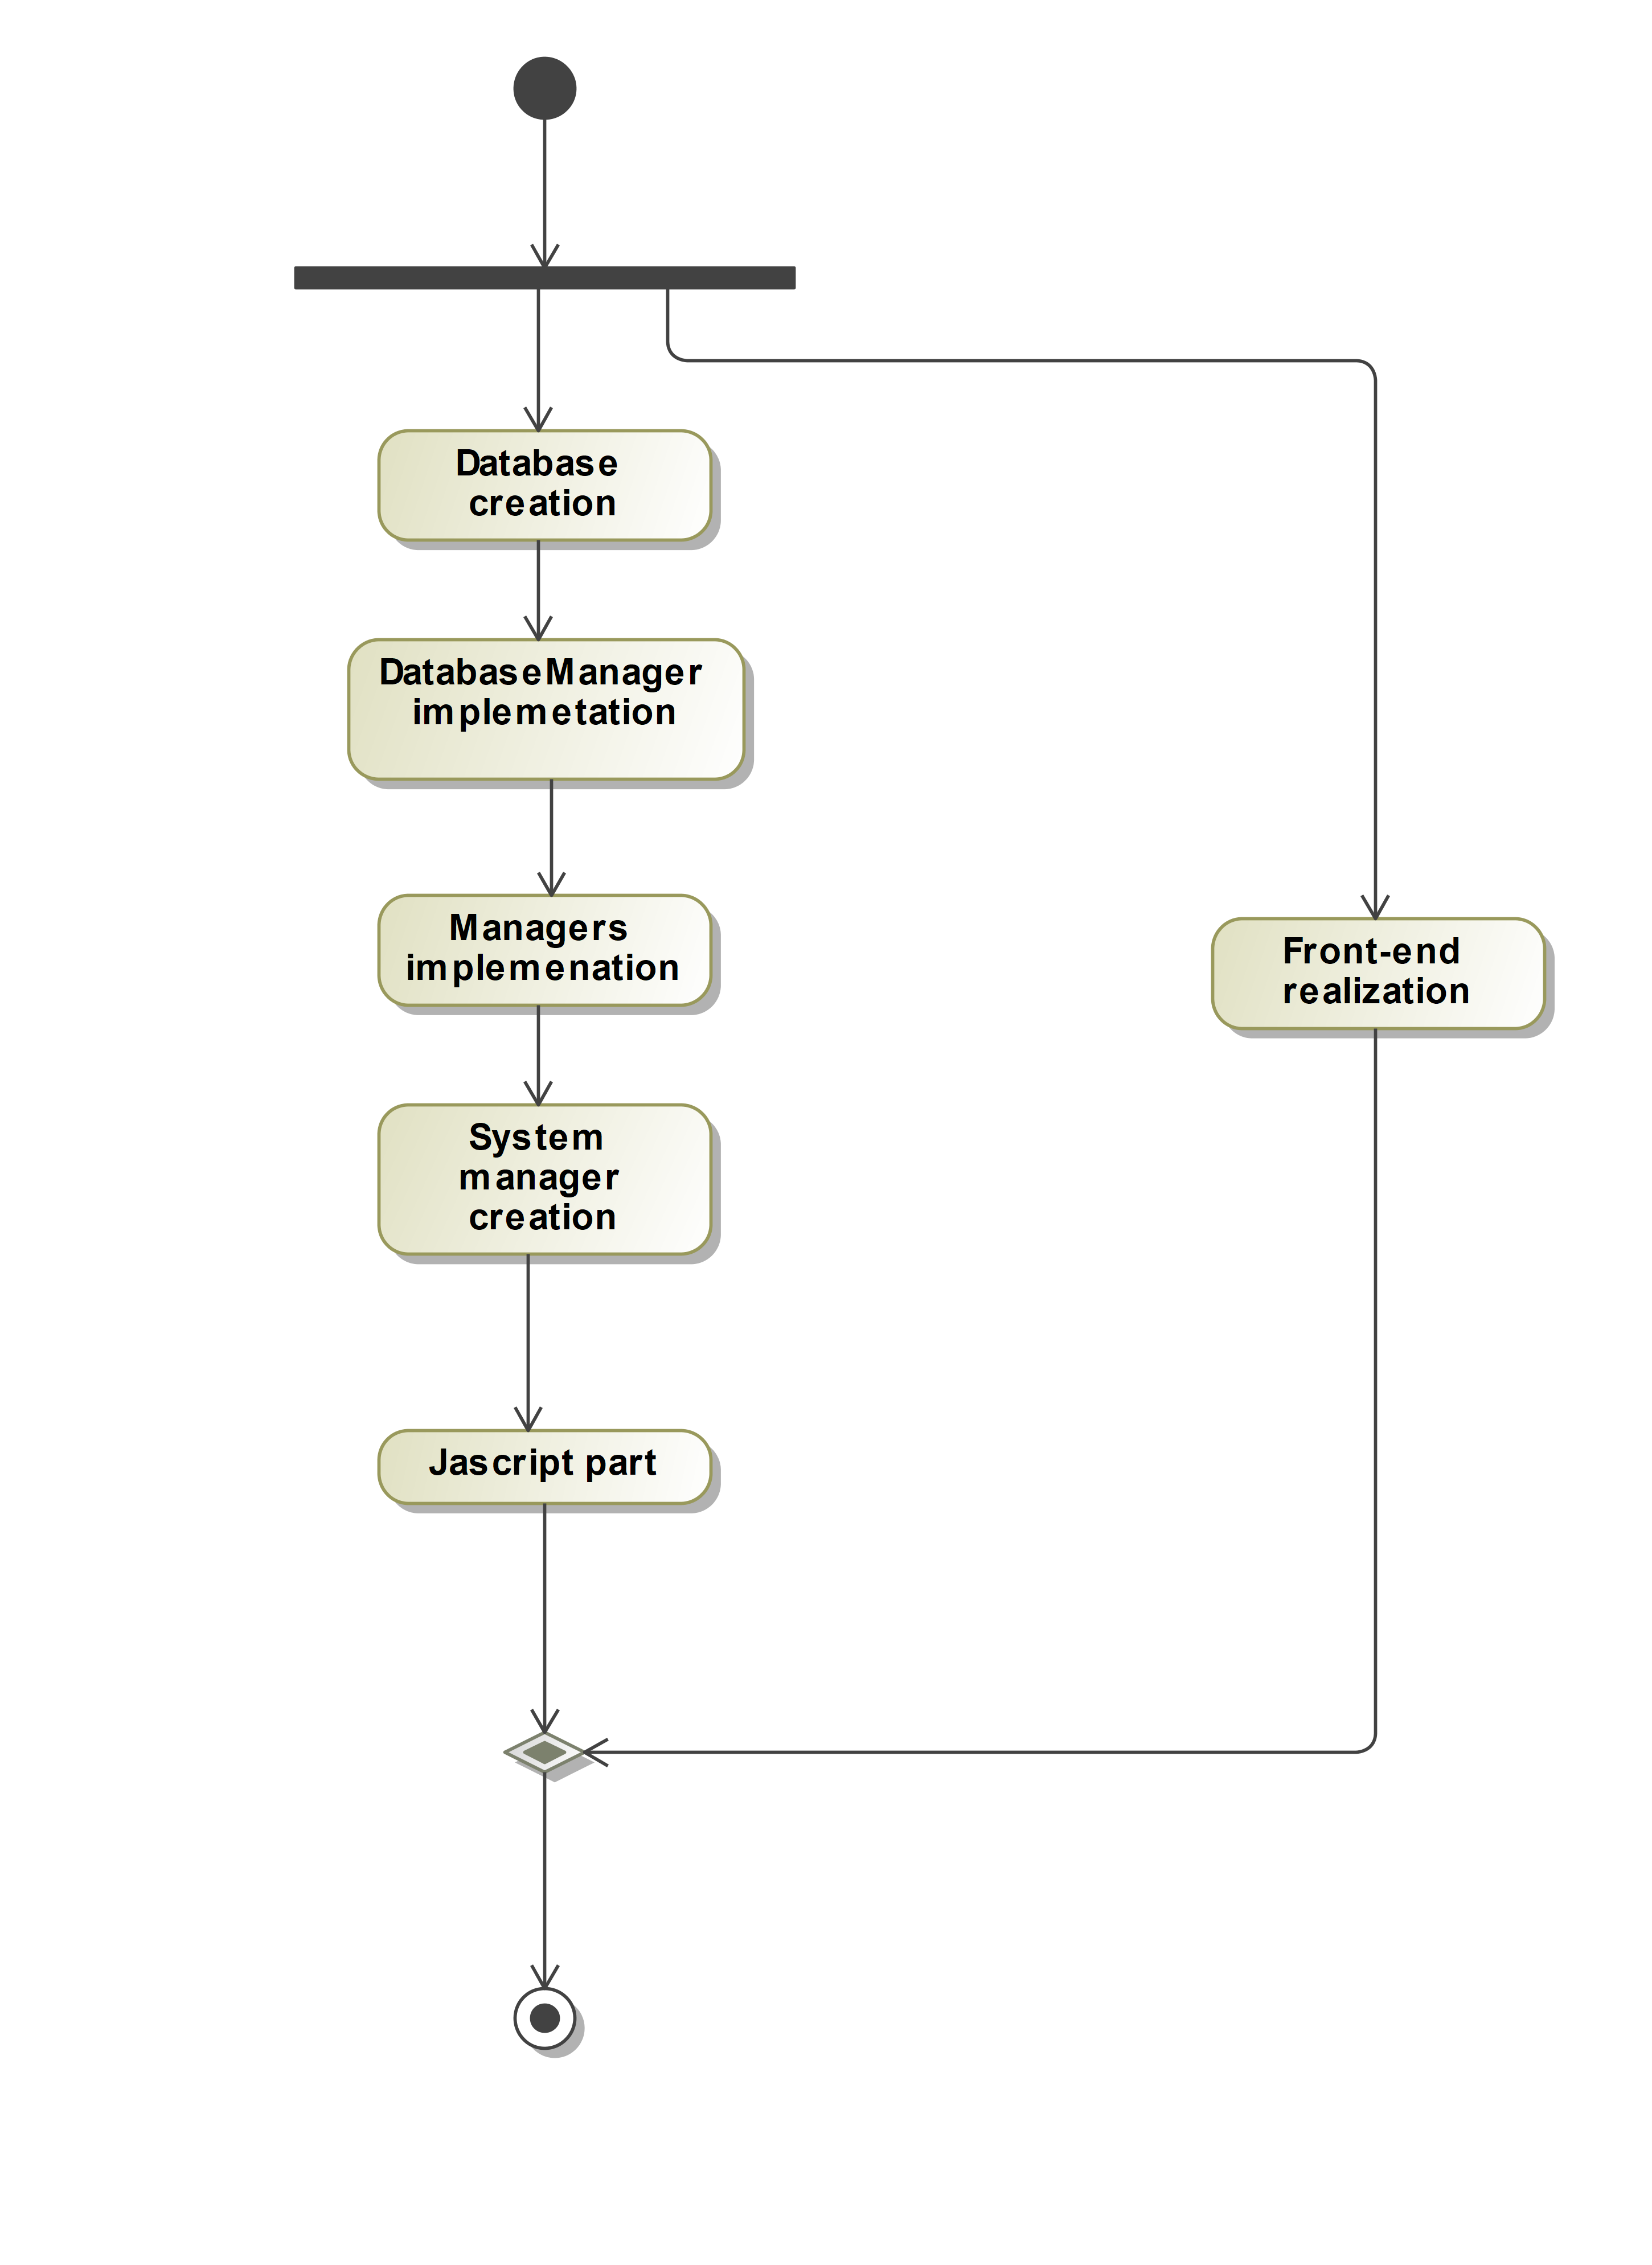
\includegraphics[width=0.7\linewidth]{Images/Tasks}
	\caption{Tasks flow}
	\label{Tasks flow}
\end{figure}

\subsection{Testing}

\paragraph{Unit tests:}
Tests of the system components will be done on the single piece of code in order to unsure the reliability of their behavior.
By definition, Unit tests should have no dependencies on code outside the unit tested.

\paragraph{Integration tests:}
When SafeStreets will be realized, the whole system will be tested to check if different pieces of the modules are working together.

